\documentclass[10pt,aspectratio=169]{beamer}
\usepackage{amsmath,amssymb}
\usepackage{booktabs}
\usepackage{graphicx}
\graphicspath{{../methods/}}  % figures: docs/robust/methods (report/methods in the working copy)

% ---- a plain look, colours of the methods figures --------------------------
\usetheme{default}
\definecolor{ink}{HTML}{222222}
\definecolor{muted}{HTML}{666666}
\definecolor{accent}{HTML}{0072B2}
\definecolor{warm}{HTML}{D55E00}
\definecolor{good}{HTML}{009E73}
\setbeamercolor{frametitle}{fg=accent}
\setbeamercolor{title}{fg=accent}
\setbeamercolor{normal text}{fg=ink}
\setbeamercolor{structure}{fg=accent}
\setbeamercolor{alerted text}{fg=warm}
\setbeamertemplate{navigation symbols}{}
\setbeamertemplate{itemize items}[circle]
\setbeamerfont{frametitle}{size=\large,series=\bfseries}
\setbeamertemplate{footline}{\hfill{\color{muted}\scriptsize\insertframenumber\ /\ \inserttotalframenumber}\hspace{6pt}\vspace{4pt}}
\newcommand{\opt}[1]{\texttt{-{}-#1}}
\newcommand{\take}[1]{\vfill{\color{accent}\bfseries #1}}

\title{Relatedness in PCA\\[2pt]\normalsize and how to deal with it}
\subtitle{PCAone \opt{robust}: small samples, biobanks and admixed relatives}
\author{relatePCA}
\date{\today}

\begin{document}

\begin{frame}
\titlepage
\end{frame}

% ============================================================== the problem
\section{The problem}

\begin{frame}{Relatives add covariance that is not ancestry}
\begin{columns}[T]
\column{0.5\textwidth}
\begin{itemize}
  \item PCA of genotypes is a PCA of their covariance between individuals.
  \item Relatives share alleles identical by descent:
    $\operatorname{Cov}(g_i,g_j)=4\phi_{ij}\,\pi(1-\pi)$, on top of ancestry.
\end{itemize}
\column{0.48\textwidth}
\begin{itemize}
  \item A family is a small, tight cluster: PCA spends components on it.
  \item Goal: \textbf{every individual in-sample} (no projection), PCs not
    shaped by close relatives (2nd degree and closer).
\end{itemize}
\end{columns}
\vspace{12pt}
\centering
{\scriptsize\color{ink}\makebox[\linewidth]{%
\makebox[0.166\linewidth]{reference truth}\makebox[0.166\linewidth]{\textbf{standard PCA}}%
\makebox[0.166\linewidth]{aarobust-kin}\makebox[0.166\linewidth]{detect-white}%
\makebox[0.166\linewidth]{cswhite}\makebox[0.166\linewidth]{frkin}}}\\[3pt]
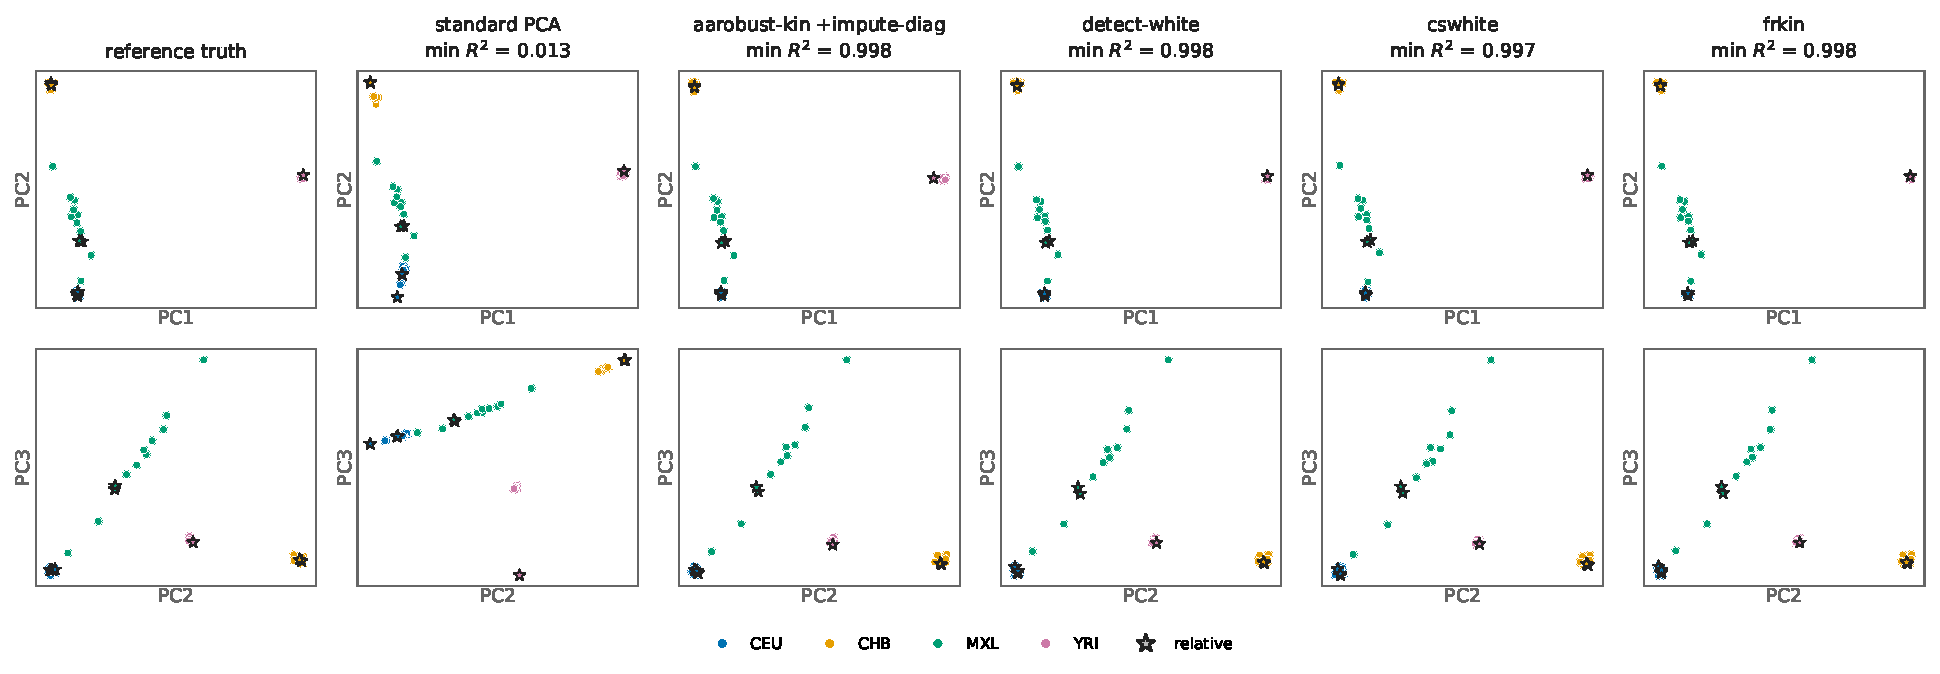
\includegraphics[width=\linewidth,trim=0 0 0 172bp,clip]{overview_pcs.pdf}\\[-1pt]
{\scriptsize\color{muted} PC2 vs PC3; admixTjeck2, 10 per population + 8 relatives
(stars). Standard PCA loses the 3rd axis (min $R^2=0.013$ against the reference
truth); every robust mode recovers it ($\ge0.997$).}
\end{frame}

\begin{frame}{Two regimes}
\begin{columns}[T]
\column{0.48\textwidth}
\textbf{Small samples} (a few individuals per population)
\begin{itemize}
  \item one family can capture an ancestry axis;
  \item standard PCA fails in 79\% of benchmark runs (min $R^2<0.95$).
\end{itemize}
\vspace{4pt}
\textbf{Large samples}
\begin{itemize}
  \item the top axes survive;
  \item relatives are misplaced;
  \item the PCs just beyond the ancestry axes become \emph{family axes}.
\end{itemize}
\column{0.5\textwidth}
\small
\begin{tabular}{@{}lcc@{}}
\toprule
$N=2000$, 30\% in families & standard & robust \\
\midrule
top 4 axes, min $R^2$ & 0.956 & 0.957 \\
relatives' error & 0.49 & 0.12 \\
family axes (of 16 extra PCs) & 16 & 0 \\
largest family share $\eta^2$ & 0.91 & 0.17 \\
\bottomrule
\end{tabular}\\[4pt]
{\scriptsize\color{muted} Simulated, 5 populations ($F_{ST}$ 0.05--0.002)
+ admixed; truth: PCA of a separate reference panel.}
\end{columns}
\take{Small N: an accuracy problem. Large N: a placement and extra-PC problem.}
\end{frame}

\begin{frame}{The usual fixes and what they cost}
\begin{itemize}
  \item \textbf{Remove relatives} (keep one per family): loses individuals and
    their PCs; needs a pedigree or a relatedness screen first.
  \item \textbf{PC-AiR}: PCA of an unrelated subset, relatives \emph{projected}:
    relatives are not in-sample, and projection shrinks them.
  \item \textbf{KING-robust screen}: fine within an unadmixed population, biased
    across populations and for admixed individuals (later).
\end{itemize}
\vspace{6pt}
\textbf{What we want instead}
\begin{itemize}
  \item a decomposition of the individual-by-individual matrix into
    \emph{structure} (low rank) and \emph{relatives} (sparse);
  \item a kinship threshold, not a tuning constant: $\tau=2^{-3.5}\approx0.088$,
    between 2nd (0.125) and 3rd degree (0.0625);
  \item PCs from the structure, or from a matrix in which families are
    \emph{whitened} (down-weighted to their effective size).
\end{itemize}
\end{frame}

% ============================================================== small N
\section{The small-$N$ problem}

\begin{frame}{Small $N$ I: the diagonal}
\begin{columns}[T]
\column{0.38\textwidth}
\begin{itemize}
  \item The GRM diagonal is a structure part plus heterozygosity noise.
  \item At $n=5$ per population the noise dominates, and it differs by
    population (YRI highest).
  \item The uneven diagonal acts as a population indicator: PCA spends an axis
    on it --- \emph{even without relatives}.
  \item Fix: treat the diagonal as \textbf{unobserved}, impute it from the
    off-diagonal entries (\opt{impute-diag}).
\end{itemize}
\column{0.6\textwidth}
\centering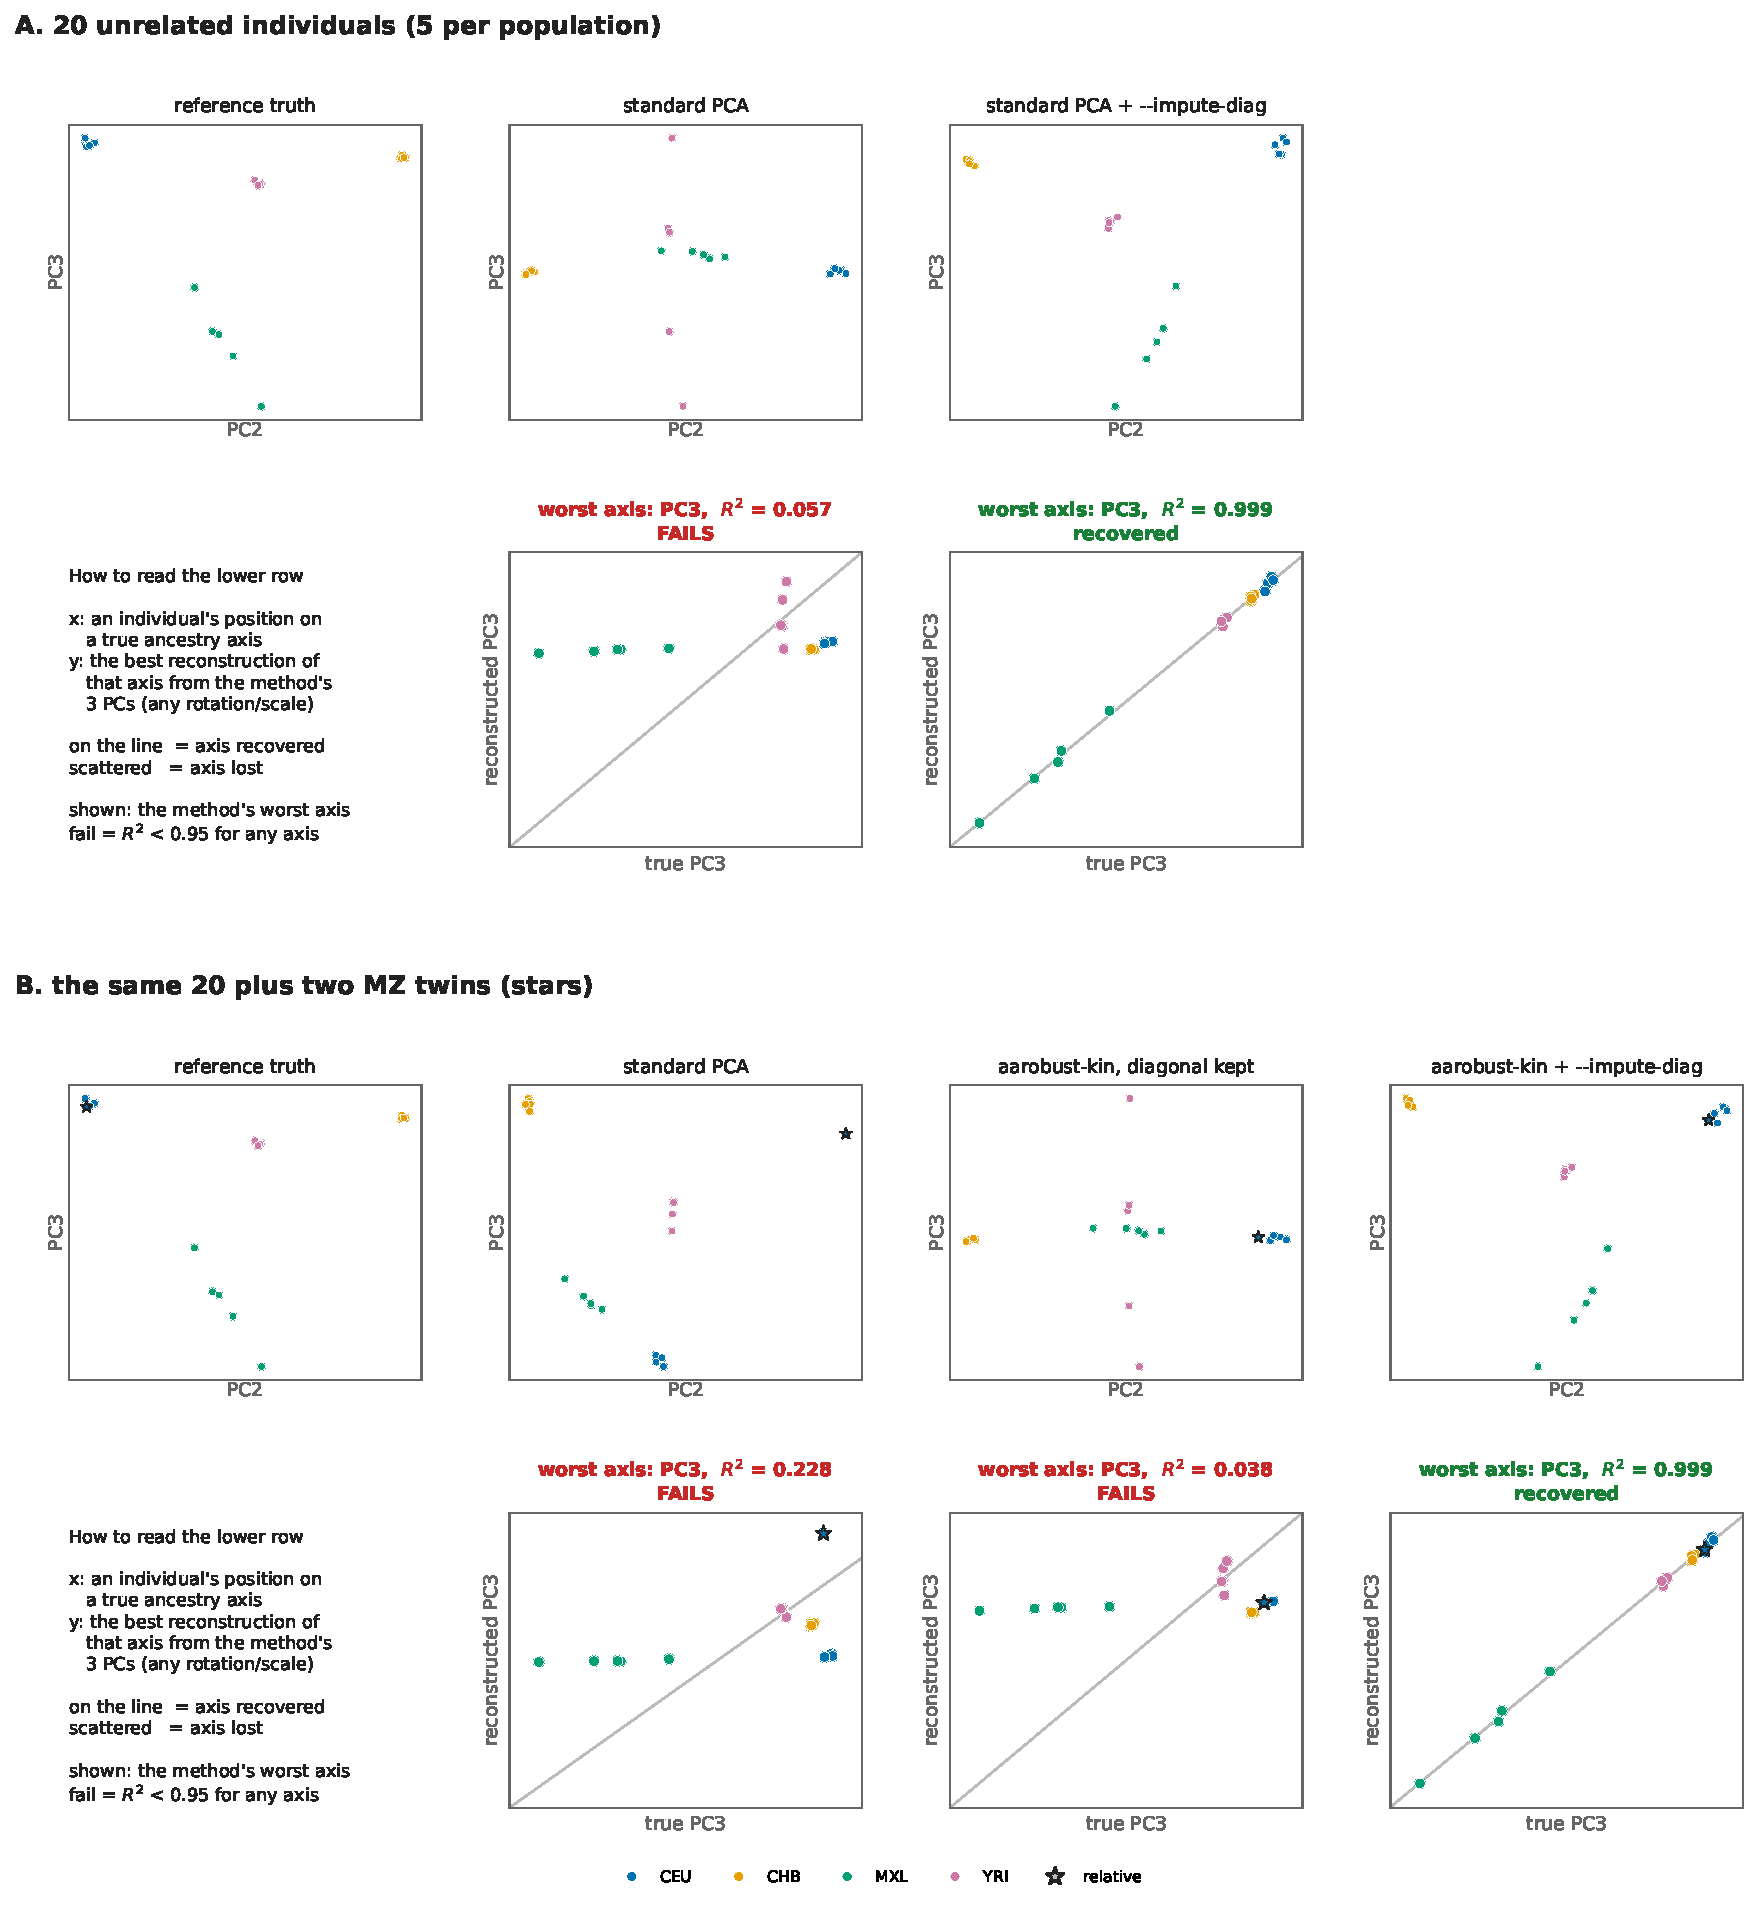
\includegraphics[height=0.72\textheight,width=\linewidth,keepaspectratio]{smalln_fail.pdf}
\end{columns}
\take{At $n=5$, mean min $R^2$: diagonal kept 0.022 (unrelated only) / 0.018 (with relatives); imputed 0.985 / 0.989.}
\end{frame}

\begin{frame}{Small $N$ II: centring leaks the diagonal into every entry}
\begin{columns}[T]
\column{0.52\textwidth}
\begin{itemize}
  \item The GRM is built from centred genotypes: $C=JAJ$, $J=I-\mathbf 1\mathbf 1'/N$.
  \item A diagonal noise term becomes
  \[ JDJ = D-\frac{d\mathbf 1'+\mathbf 1 d'}{N}+\frac{\bar d}{N}\mathbf 1\mathbf 1' \]
  so $C_{ij}$ picks up $-(d_i+d_j)/N$.
  \item Rows of $C$ sum to zero: freeing the diagonal frees nothing.
  \item Undo it: $A = C+u\mathbf 1'+\mathbf 1u'+(\mu'\mu/M)\mathbf 1\mathbf 1'$,
    $u=X_c\mu/M$ --- needs $f$ \emph{and} one number per individual.
\end{itemize}
\column{0.46\textwidth}
\small
\begin{tabular}{@{}lc@{}}
\toprule
rank fit, diagonal free, on & failures, $n=5$ \\
\midrule
GRM, scaled + \textbf{centred} & 82\% \\
GRM, scaled, \textbf{not centred} & 0\% \\
CS matrix (raw, not centred) & 0\% \\
PCP on the centred GRM & 2.5\% \\
\bottomrule
\end{tabular}\\[4pt]
{\scriptsize\color{muted} Scaling by $2f(1-f)$ makes no difference; centring
does. PCP survives only because its fit ends up full rank.}
\end{columns}
\take{Work on the uncentred matrix (or restore it), with the diagonal free.}
\end{frame}

% ============================================================== methods
\section{Methods}

\begin{frame}{Robust PCA of the GRM with a kinship threshold (\texttt{aarobust-kin})}
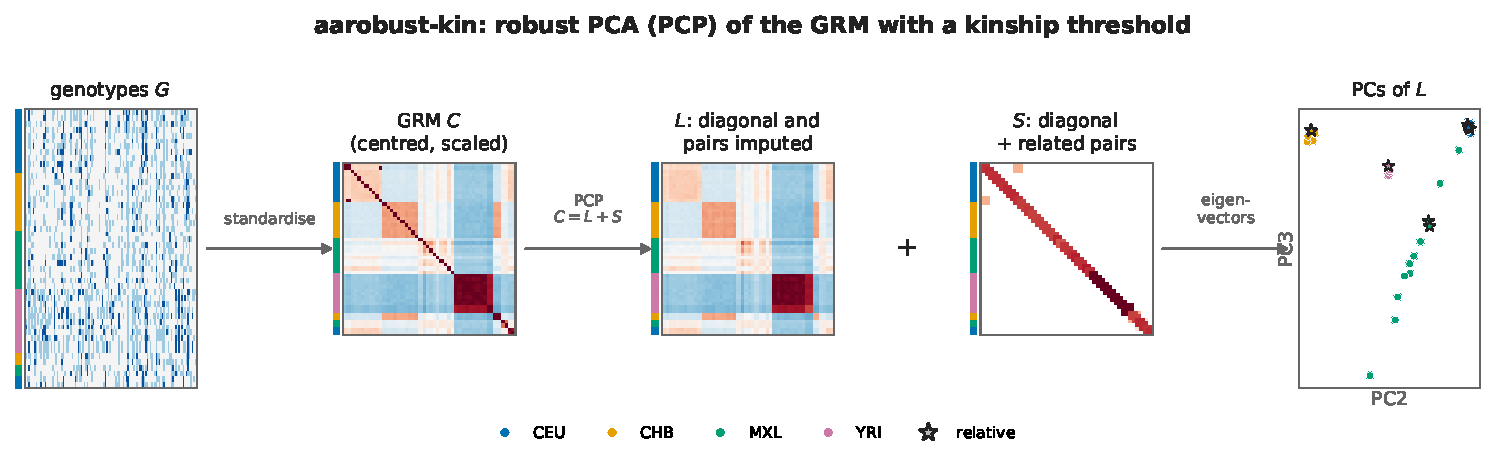
\includegraphics[width=\linewidth,trim=0 0 0 1.05cm,clip]{ga_aarobust.pdf}
\begin{itemize}
  \item PCP $C=L+S$: diagonal always in $S$; a pair enters $S$ only if its
    kinship exceeds $\tau$ (and it passes a screen) --- no $\lambda$, no rank.
  \item Needs the full spectrum in every iteration ($N^3$): 31\,s at $N=1000$,
    248\,s at $N=2000$. Partial (IRAM) solves do not help: $L$ ends up full rank.
\end{itemize}
\end{frame}

\begin{frame}{\texttt{dwg}: detect, then whiten (the default)}
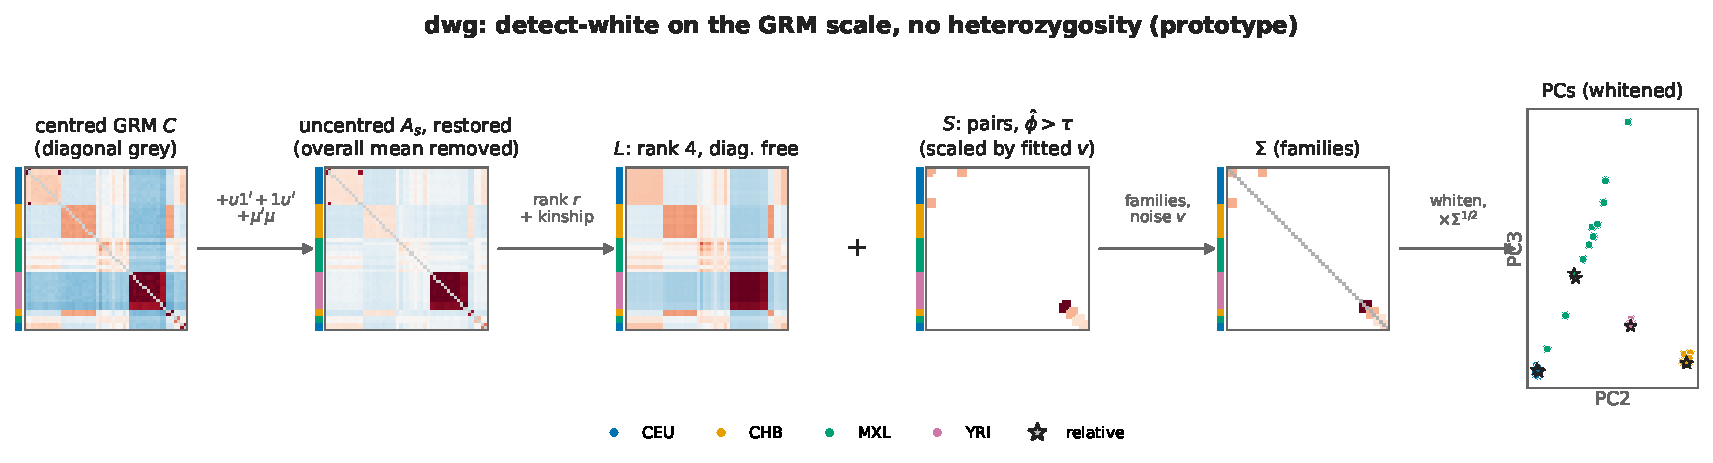
\includegraphics[width=\linewidth,trim=0 0 0 1.05cm,clip]{ga_dwg.pdf}
\begin{itemize}
  \item Uncentred, SNP-standardised Gram; low-rank fit with the diagonal free;
    kinship scaled by the \emph{fitted} noise $v_i$ (no HWE within individuals).
  \item Whitening $\Sigma=v^{1/2}(I+2\Psi)v^{1/2}$: a family counts as its effective
    number of individuals. Only the top $r$ eigenvectors per step.
\end{itemize}
\end{frame}

\begin{frame}{Choosing the rank without knowing $K$}
\begin{columns}[T]
\column{0.5\textwidth}
\begin{itemize}
  \item Raise the rank while the next eigenvalue exceeds the noise edge
    $2\sigma\sqrt N$; $k$ is only an upper bound.
  \item \textbf{Family axes}: an eigenvector resting on $<4$ individuals
    ($n_{\text{eff}}=1/\sum u_i^4$) with a related pair among them is a family,
    not structure: its pairs become candidates, the rank is not raised.
  \item Ancestry axes rest on whole populations ($n_{\text{eff}}$ 14--49 at
    $n=20$), family axes on 2--3 individuals.
\end{itemize}
\column{0.48\textwidth}
\small
\begin{tabular}{@{}lcc@{}}
\toprule
 & KING screen & \texttt{dwg} \\
\midrule
failures $k=10$, $n=5$ & 6.7\% & 1.7\% \\
failures $k=10$, $n=10$ & 6.7\% & 0\% \\
relatives' error ($k=10$) & 0.25 & 0.09 \\
runs changed by $k$ (of 240) & 12 & 2 \\
\bottomrule
\end{tabular}\\[4pt]
{\scriptsize\color{muted} 12 scenarios incl.\ relatives of different
ancestry, 5 replicates; $k=3$ and $k=10$ with true $K-1=3$.}
\end{columns}
\end{frame}

\begin{frame}{Whiten, do not just impute}
\begin{columns}[T]
\column{0.5\textwidth}
\begin{itemize}
  \item Alternative: PCs of the Gram with the related pairs and the diagonal
    imputed. As accurate on the top PCs, and all $k$ PCs exist.
  \item But imputation leaves each relative a full individual: sibs keep
    near-identical correlations with everyone else.
  \item Whitening corrects the weighting.
\end{itemize}
\column{0.48\textwidth}
\small
\begin{tabular}{@{}lcc@{}}
\toprule
$N=2000$, PCs 5--20 & family axes & median $\eta^2$ \\
\midrule
standard PCA & 16 of 16 & 0.92 \\
imputed pairs + diagonal & 0 & 0.37 \\
\textbf{whitening} & \textbf{0} & \textbf{0.21} \\
\bottomrule
\end{tabular}\\[4pt]
{\scriptsize\color{muted} $\eta^2$: share of a PC's variance explained by
family membership (30\% of the sample in families).}
\end{columns}
\end{frame}

% ============================================================== admixed
\section{Kinship for admixed individuals}

\begin{frame}{Admixed I: KING is not structure-free}
\begin{columns}[T]
\column{0.44\textwidth}
\begin{itemize}
  \item KING-robust corrects for heterozygosity differences between
    populations: valid for two individuals from the \emph{same unadmixed}
    population.
  \item Relatives of different ancestry: pulled \textbf{down}.
  \item Admixed individuals of similar ancestry: pulled \textbf{up}.
  \item Below the 0.04 screen a pair can never be called related.
\end{itemize}
\column{0.54\textwidth}
\small
\begin{tabular}{@{}lcc@{}}
\toprule
true pair (kinship) & KING & evalAdmix \\
\midrule
grandparent -- grandchild$^a$ (0.125) & \alert{$-0.013$} & 0.085 \\
aunt -- nephew$^b$ (0.125) & \alert{0.017} & 0.089 \\
half-sibs$^c$ (0.125) & 0.069 & 0.089 \\
parent -- child$^d$ (0.25) & 0.187 & 0.236 \\
\bottomrule
\end{tabular}\\[4pt]
{\scriptsize\color{muted} $^a$YRI and $\tfrac14$ YRI; $^b$CHB and CHB/YRI;
$^c$CEU$\times$CHB and CEU$\times$YRI; $^d$CEU$\times$YRI child. Lowest values
over 5 replicates; relatives from real admixTjeck2 genotypes with recombination.}
\end{columns}
\take{KING-only screening missed 40--47\% of these cross-ancestry 2nd-degree pairs.}
\end{frame}

\begin{frame}{Admixed II: individual allele frequencies}
\begin{itemize}
  \item Predict each genotype from the individual's own ancestry: individual
    allele frequency $\pi_{is}$; relatedness is what the prediction leaves.
  \item PC-Relate, PCAngsd and evalAdmix are \textbf{one estimator}: the
    correlation of residuals estimates $2\phi$. They differ only in
    \begin{enumerate}
      \item where $\hat\pi$ comes from (PCs or an admixture model),
      \item the denominator (model or observed variance),
      \item whether the pair's own genotypes were used to build $\hat\pi$.
    \end{enumerate}
  \item The number of PCs matters most: use $K-1$ (plus intercept). Too many PCs
    absorb the relatives themselves.
\end{itemize}
\vspace{2pt}
{\small
\begin{tabular}{@{}lccc@{}}
\toprule
RMSE & PC-Relate & evalAdmix (EM) & PCAone \opt{evaladmix} \\
\midrule
unrelated pairs & \textbf{0.00330} & 0.00378 & 0.00386 \\
related pairs & 0.00358 & 0.00292 & \textbf{0.00251} \\
\bottomrule
\end{tabular}}
\end{frame}

\begin{frame}{Admixed III: an admixture-aware screen in \texttt{dwg}}
\begin{columns}[T]
\column{0.5\textwidth}
\begin{enumerate}
  \item First fit with the KING screen (a safe guard for the early, low-rank
    steps).
  \item evalAdmix kinship from the fit's \emph{structure} axes (family axes
    left out) $\to$ candidates $>0.04$.
  \item evalAdmix alone flags unrelated admixed pairs of similar ancestry at
    small $N$ (two MXL: 0.113). Confirm by \textbf{IBD}: $k_0<0.8$
    (unrelated $\approx1$, 2nd degree $\approx0.5$).
  \item Refit; stop when the pairs no longer change.
\end{enumerate}
\column{0.48\textwidth}
\small
\begin{tabular}{@{}lcc@{}}
\toprule
recall, $k=10$ & KING & \texttt{dwg} \\
\midrule
$n=5$ & 88\% & 95\% \\
$n=10$ & 88\% & 96\% \\
$n=20$ & 86\% & 97\% \\
$n=40$ & 90\% & 100\% \\
false pairs & 0 & 0 \\
\bottomrule
\end{tabular}\\[4pt]
{\scriptsize\color{muted} Same accuracy as an evalAdmix screen with the true
$K-1$ --- without knowing $K$.}
\end{columns}
\end{frame}

\begin{frame}{Admixed IV: final relatedness, $(k_0,k_1,k_2)$}
\begin{columns}[T]
\column{0.46\textwidth}
\begin{itemize}
  \item Kinship alone cannot separate parent--offspring from full sibs (both
    $\tfrac14$); $k_0$ can (0 vs $\tfrac14$).
  \item Allele-level likelihood with \textbf{$\pi_i\neq\pi_j$}: pooling the two
    frequencies reports a parent--offspring pair as 83\% unrelated.
  \item Allele frequencies from the final PCs, the pair's \textbf{whole family
    left out}; projected Newton (EM stalls at $k_0=0$).
\end{itemize}
\column{0.52\textwidth}
\small
\begin{tabular}{@{}lccc@{}}
\toprule
$N=2000$ (simulated) & kinship & $k_0$ & $k_1$ \\
\midrule
parent--offspring & 0.251 & 0.000 & 0.996 \\
full sibs & 0.250 & 0.250 & 0.500 \\
2nd degree & 0.126 & 0.504 & 0.490 \\
MZ & 0.500 & 0.000 & 0.000 \\
\bottomrule
\end{tabular}\\[4pt]
{\scriptsize\color{muted} Written to \texttt{.relpairs}. At $N=47$ (real
genotypes): PO and sibs separated; 2nd degree $\approx0.02$ too high.}
\end{columns}
\end{frame}

% ============================================================== evidence
\section{Evidence}

\begin{frame}{Real LD and real panels}
\begin{columns}[T]
\column{0.52\textwidth}
\textbf{HAPNEST} (synthetic biobank, realistic LD, 6 ancestries), $N=5000$
\vspace{2pt}

\scriptsize
\begin{tabular}{@{}lccc@{}}
\toprule
 & standard & detect-white & \textbf{dwg} \\
\midrule
min $R^2$ (5 axes) & 0.9987 & 0.9977 & \textbf{0.9988} \\
relatives' error & 0.048 & 0.028 & \textbf{0.019} \\
family axes & 15/15 & 0 & 0 \\
recall & -- & 97.3\% & \textbf{98.3\%} \\
cross-anc.\ grandparent & -- & 66\% & \textbf{87\%} \\
time & 14\,s & 100\,s & 21\,s \\
\bottomrule
\end{tabular}
\column{0.44\textwidth}
\textbf{1000 Genomes} (CEU, CHB, YRI, ASW), $n=5$--20
\vspace{2pt}

\scriptsize
\begin{tabular}{@{}lcc@{}}
\toprule
 & failures & recall \\
\midrule
standard & 27\% / 10\% / 0 & -- \\
aarobust-kin & 0 & 78--84\% \\
detect-white & 0 & 78--83\% \\
\textbf{dwg} & \textbf{0} & \textbf{90--96\%} \\
\bottomrule
\end{tabular}\\[4pt]
{\scriptsize\color{muted} Every pair \texttt{dwg} missed on HAPNEST had
realised kinship $<\tau$. The extra 1000G pairs are real relatives in the
panel (e.g.\ NA20317/NA20318).}
\end{columns}
\end{frame}

% ============================================================== scale
\section{Large and very large $N$}

\begin{frame}{Large $N$: no $N\times N$ matrix}
\begin{columns}[T]
\column{0.5\textwidth}
\begin{itemize}
  \item Operator engine: each iteration is one pass $G(G'V)$ with a few vectors;
    in-core or out-of-core.
  \item Candidates: bit-packed KING over all pairs (popcounts); exact
    GRM-scale entries for them in one weighted pass.
  \item Family-axis checks by one product with unit vectors.
\end{itemize}
\column{0.48\textwidth}
\small
\begin{tabular}{@{}lcc@{}}
\toprule
16 threads & \texttt{dwg} & standard \\
\midrule
$N=1000$ & 1.1\,s & -- \\
$N=5000$ & 4.7\,s & 3.5\,s \\
$N=20{,}000$ in-core & 26.5\,s & 24\,s \\
$N=20{,}000$ out-of-core & 109\,s & 29\,s \\
\bottomrule
\end{tabular}\\[4pt]
{\scriptsize\color{muted} Dense engine (\texttt{dwg}): 10.7\,s at
$N=2000$; \texttt{aarobust-kin} 248\,s.}
\end{columns}
\end{frame}

\begin{frame}{Very large $N$: finding the relatives with a sketch}
\centering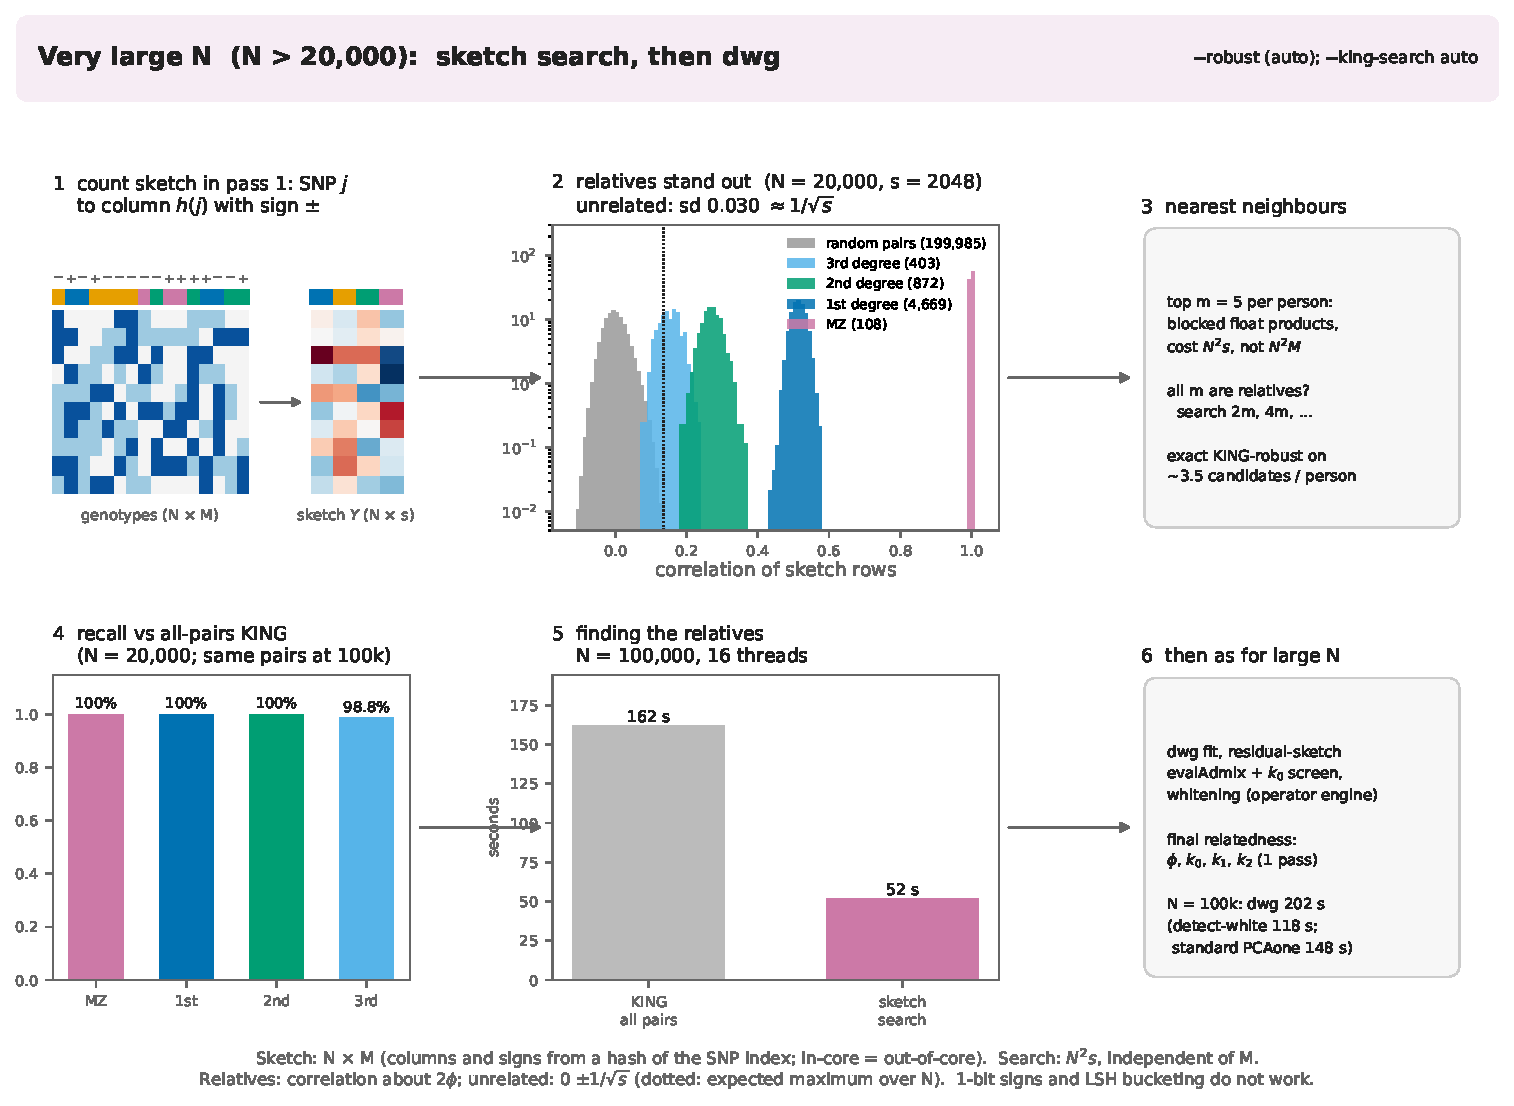
\includegraphics[height=0.74\textheight]{regime_verylarge.pdf}\\[2pt]
{\small Count sketch in the first pass ($N\times M$); nearest neighbours $N^2s$,
independent of $M$; exact KING on $\sim$3.5 candidates per person.
$N=100{,}000$: the same 27{,}880 pairs as all-pairs KING, 52\,s instead of 162\,s.}
\end{frame}

% ============================================================== GL
\section{Genotype likelihoods}

\begin{frame}{Genotype likelihoods (\texttt{-G})}
\begin{columns}[T]
\column{0.5\textwidth}
\begin{itemize}
  \item Posterior means shrink towards the prior --- more at low depth.
  \item \textbf{Deshrink}: $x=2f+(E-2f)/\rho_i$, $\rho_i$ the genotype
    reliability; off-diagonal products $\approx$ unbiased, extra noise on
    the free diagonal.
  \item Kinship decisions $/\sqrt{\rho_i\rho_j}$; screen with KING from expected
    counts; $k_0$ and final $(k_0,k_1,k_2)$ from the likelihoods.
  \item One round with the HWE prior beats iterated (PCAngsd-style) priors.
\end{itemize}
\column{0.48\textwidth}
\small
\begin{tabular}{@{}lcc@{}}
\toprule
failures & $n=10$ & $n=5$ \\
\midrule
true genotypes & 0 & 0 \\
\textbf{GL, 8$\times$} & \textbf{0} & 6\% \\
\textbf{GL, 4$\times$} & \textbf{0} & 12.5\% \\
\textbf{GL, 2$\times$} & \textbf{0} & 19\% \\
standard GL PCA, 4$\times$ & 100\% & 100\% \\
\bottomrule
\end{tabular}\\[4pt]
{\scriptsize\color{muted} Simulated reads (1\% error) on admixTjeck2, 54k SNPs.
At $1\times$ nothing works with 5 per population.}
\end{columns}
\end{frame}

% ============================================================== use
\section{Using it}

\begin{frame}[fragile]{Using it}
\footnotesize
\begin{verbatim}
PCAone -b data -k K-1 --robust              # dwg, any N
PCAone -b data -k 10 --robust -m 2          # out-of-core
PCAone -G data.beagle.gz -k K-1 --robust    # genotype likelihoods
PCAone -b data -k 3 --robust --impute-diag  # aarobust-kin (PCP)
PCAone -b data -k K-1 --robust --kinship pairs.kin0   # known pedigree
\end{verbatim}
\normalsize
\vspace{4pt}
\begin{itemize}
  \item \texttt{.eigvecs / .eigvals}: the robust PCs (a generous $k$ is safe).
  \item \texttt{.relpairs}: \texttt{KING}, \texttt{KIN\_DETECT} (decides the
    pair), \texttt{KINSHIP K0 K1 K2} (final, from the final PCs),
    \texttt{KIN\_EVALADMIX}.
  \item Code and the full methods document: branch \texttt{robust-relatives},
    \texttt{docs/robust/README.md}.
\end{itemize}
\end{frame}

\begin{frame}{Summary}
\begin{itemize}
  \item Relatives distort PCA differently by sample size: a lost axis at small
    $N$, misplaced relatives and family axes at large $N$.
  \item At small $N$ the GRM diagonal is a second, independent problem --- and
    centring spreads it into every entry. Work uncentred, diagonal free.
  \item \texttt{dwg}: detect related pairs with a kinship threshold, then
    whiten. No HWE assumption, $k$ only an upper bound, all individuals
    in-sample; from 20 individuals to 100{,}000.
  \item Admixed relatives: KING misses them; an evalAdmix screen from the
    structure axes, confirmed by IBD, finds them.
  \item Final relatedness from the final PCs: $(k_0,k_1,k_2)$ with $\pi_i\ne\pi_j$
    and leave-the-family-out frequencies.
\end{itemize}
\vspace{4pt}
\textbf{Open:} missing genotypes; parent--offspring $k_2$ with low-depth GL;
first cousins at $\sim$5 per population.
\end{frame}

% ============================================================== backup
\appendix
\begin{frame}{Backup: the three regimes and the engines}
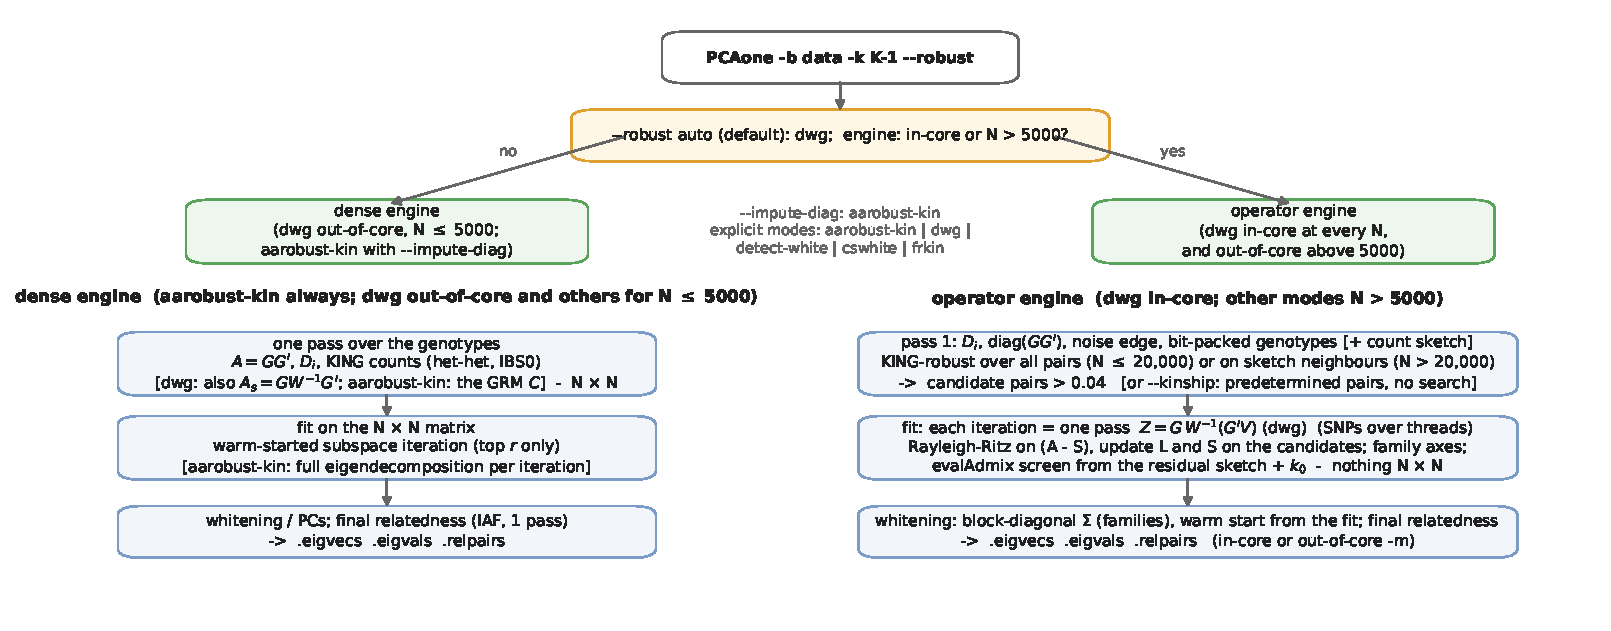
\includegraphics[width=\linewidth]{engines.pdf}
\end{frame}

\begin{frame}{Backup: building blocks}
\begin{itemize}
  \item KING-robust:
  $\phi^{\mathrm{KING}}_{ij}=\dfrac{N^{\mathrm{het,het}}_{ij}-2N^{\mathrm{IBS0}}_{ij}}{2m_{ij}}
  +\dfrac12-\dfrac{N^{\mathrm{het}}_i+N^{\mathrm{het}}_j}{4m_{ij}}$,
  $m_{ij}=\min(N^{\mathrm{het}}_i,N^{\mathrm{het}}_j)$.
  \item Structure-adjusted kinship from a residual $R=A-L$:
  $\hat\phi_{ij}=R_{ij}/(2\sqrt{v_iv_j})$.
  \item Noise edge: $2\sigma\sqrt N$, $\sigma^2=\sum_s\big(\mathrm E[g^2]^2-(2f_s)^4\big)/(w_s^2M^2)$.
  \item IBD likelihood per site (allele level): IBD0 $g_i\sim\mathrm{HWE}(\pi_i)$,
    $g_j\sim\mathrm{HWE}(\pi_j)$; IBD1 shared allele $\sim\tfrac12(\pi_i+\pi_j)$;
    IBD2 $g_i=g_j\sim\mathrm{HWE}(\tfrac12(\pi_i+\pi_j))$.
\end{itemize}
\end{frame}

\end{document}
